%
% CSE Electronic Homework Template
% Last modified 8/20/2019 by Jeremy Buhler

\documentclass[11pt]{article}
\usepackage[left=0.7in,right=0.7in,top=1in,bottom=0.7in]{geometry}
\usepackage{fancyhdr} % for header
\usepackage{graphicx} % for figures
\usepackage{amsmath}  % for extended math markup
\usepackage{amssymb}
\usepackage{tikz}
\usepackage[noend]{algpseudocode} % for pseudocode
\usepackage[plain]{algorithm} % float environment for algorithms

\usetikzlibrary{graphs.standard}

%%%%%%%%%%%%%%%%%%%%%%%%%%%%%%%%%%%%%%%%%%%%%%%%%%%%%%%%%%%%%%%%%%%%%%
% STUDENT: modify the following fields to reflect your the current
% homework number.  Do NOT include a name or ID or other personally
% identifying info, as we will use anonymized grading in GradeScope.

\newcommand{\HomeworkNumber}{5}

%%%%%%%%%%%%%%%%%%%%%%%%%%%%%%%%%%%%%%%%%%%%%%%%%%%%%%%%%%%%%%%%%%%%%%%%
% You can pretty much leave the stuff up to the next line of %%'s alone.

% create header and footer for every page
\pagestyle{fancy}
\fancyhf{}
\rhead{\textbf{Hwk \HomeworkNumber{}}}
\cfoot{\thepage}

% preferred pseudocode style
\algrenewcommand{\algorithmicprocedure}{}
\algrenewcommand{\algorithmicthen}{}

% ``do { ... } while (cond)''
\algdef{SE}[DOWHILE]{Do}{doWhile}{\algorithmicdo}[1]{\algorithmicwhile\ #1}%

% ``for (x in y ... z)''
\newcommand{\ForRange}[3]{\For{#1 \textbf{in} #2 \ \ldots \ #3}}

% these are common math formatting commands that aren't defined by default
\newcommand{\union}{\cup}
\newcommand{\isect}{\cap}
\newcommand{\ceil}[1]{\ensuremath \left\lceil #1 \right\rceil}
\newcommand{\floor}[1]{\ensuremath \left\lfloor #1 \right\rfloor}

\newtheorem{lem}{Lemma}

%%%%%%%%%%%%%%%%%%%%%%%%%%%%%%%%%%%%%%%%%%%%%%%%%%%%%%%%%%%%%%%%%%%%%%

\begin{document}

\section{}
\subsection*{a.}
\begin{lem} 
    \label{thm:min-same}  
    At least $\frac{n}{k}$ tellers share a code.

    Suppose no code was shared by more than $\frac{n}{k} - 1$ tellers. Since there are $k$ codes, this would imply that there are at most $(\frac{n}{k} - 1)k = n - k$ tellers, contradiction the assumption that there are $n$ tellers. Therefore the assumption must be false, and a code exists which is shared by at least $\frac{n}{k}$ tellers.
\end{lem}

Suppose $m$ tellers share a code. These tellers must not be assigned to work at the same time, so within a valid shift graph, there must not be an edge between any of the $m$ tellers. Therefore a group of $m$ tellers who share the same vault code forms an independent set of size $m$ within the shift graph. By Lemma \ref{thm:min-same}, for $n$ tellers and $k$ codes, at least $\frac{n}{k}$ tellers will share a single code, so in a valid graph, there must be an independent set of size $\frac{n}{k}$.

\subsection*{b.}
The obvious reduction from ISET would be to identify the maximum independent set within the graph, assign the set a single code, remove the set from the graph, and repeat until all vertices have been removed from the graph. 
 However, this approach fails for certain graphs, where it is more efficient to eliminate a well-connected vertex earlier in the process. Consider the graph 
 \begin{figure}[H]
    \centering
    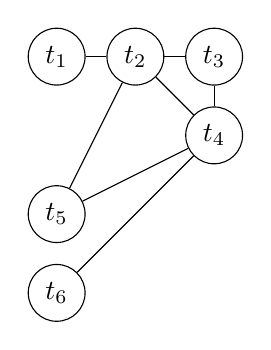
\begin{tikzpicture}
        \graph[nodes={circle, draw}] {
            "$t_1$" -- "$t_2$" -- {"$t_3$", "$t_4$"};
            "$t_4$" -- {"$t_5$", "$t_6$"};
            "$t_3$" -- "$t_4$";
            "$t_2$" -- "$t_5$";
        };
    \end{tikzpicture}
 \end{figure}

 The maximum independent set is of size $3$ and consists of tellers $t_1, t_5$ and $t_6$ or $t_1, t_3, $ and $t_6$. After eliminating each of these, the resultant graphs are 
 \begin{figure}[H]
    \centering
    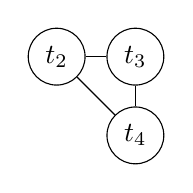
\begin{tikzpicture}
        \graph[nodes={circle, draw}] {
            "$t_2$" -- {"$t_3$", "$t_4$"};
            "$t_3$" -- "$t_4$";
        };
    \end{tikzpicture}, and
    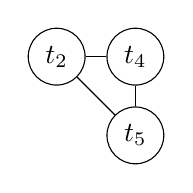
\begin{tikzpicture}
        \graph[nodes={circle, draw}] {
            "$t_2$" -- {"$t_4$", "$t_5$"};
            "$t_4$" -- "$t_5$";
        };
    \end{tikzpicture}
 \end{figure}
 Clearly, since these graphs are complete, $3$ codes would have to be assigned for the shifts to be valid, so this method assigns $4$ codes overall.

 Now consider instead choosing the smaller independent set consisting of $t_1$ and $t_4$. This yields the graph
 \begin{figure}[H]
    \centering
    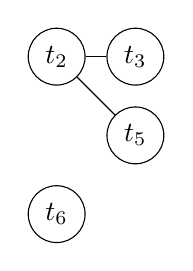
\begin{tikzpicture}
        \graph[nodes={circle, draw}] {
            "$t_2$" -- {"$t_3$", "$t_5$"};
            "$t_6$";
        };
    \end{tikzpicture}
 \end{figure}
 We can then choose the independent sets $t_3, t_5, t_6$ and $t_2$, assigning $3$ codes overall. In this case, eliminating the well-connected vertex $t_4$ also eliminated a clique within the graph, reducing the number of codes which would need to be assigned later, despite $t_4$ not being in the initial maximum independent set.


\end{document}
